\section{Zielsetzung}
\label{sec:Zielsetzung}

In diesem Versuch werden die elastischen Konstanten eines Drahtes bestimmt.
Anschließend wird das magnetische Moment eines Magneten vermessen
und die Tangentialkomponente des Erdmagnetfeldes bestimmt.

\section{Theorie}
\label{sec:Theorie}

Kräfte, die über die Oberfläche eines festen Körpers wirken, werden
Oberflächenkräfte genannt und verursachen Verformung und Volumenänderung des
Körpers.
Die einwirkende Kraft pro Fläche wird als Spannung definiert. Dabei kann die
Spannung in einen Anteil senkrecht zur Oberfläche, der
Normalspannung $\sigma$ oder Druck $P$, und einen Anteil parallel zur Oberfläche, der
Tangentialspannung $\tau$ zerlegt werden.
Bei hinreichend kleinen Deformationen sind Verformung und Volumenänderung
proportional zur wirkenden Spannung und die zugehörigen Proportionalitätsfaktoren werden
elastische Konstanten genannt. Dieser Zusammenhang wird als Hook'sches Gesetz
beschrieben.

\subsection{Elastizitätsmodule isotroper Körper}
\label{sec:Einführung}

Allgemein sind die elastischen Konstanen eines Körpers richtungsabhängig, sodass
6 Variablen für die Gestalt- und Volumenelastizität und 6 Variablen für die
Beschreibung der Deformation benötigt werden und sich damit ein
$6\times6$ Elastizitätstensor ergibt. Bei sogenannten isotropen Körpern sind
die elastischen Konstanten jedoch richtungsunabhängig, sodass der Tensor unter
Verwendung des Energieprinzips auf zwei Konstanten reduziert werden kann.

Aus praktischen Gründen werden für isotrope Körper jedoch vier
Elastizitätskonstanten eingeführt. Die Längenänderung $\increment L$ des Körpers bei
anliegender Spannung wird mit dem Elastizitätsmodul $E$ senkrecht zur
Körperoberfläche und dem Schubmodul $G$ parralel zur Körperfläche angegeben.
\begin{equation*}
  \sigma = E \cdot \frac{\increment L}{L}
%  \label{eqn:Elastizitätsmodul}
\end{equation*}
Die Volumenänderung $\increment V$ des Körpers wird mit dem
Kompressionsmodul $Q$ tangential zur
Körperoberfläche und der Poissonschen Querkontraktionszahl $\mu$ normal zur
Körperfläche angegeben.
\begin{equation*}
  P = Q \cdot \frac{\increment V}{V}
%  \label{eqn:Kompressionsmodul}
\end{equation*}

Da isotrope Körper bereits über zwei Konstanten beschrieben werden können, sind
die vier Konstanen in der Form
\begin{equation}
    E = 2 G \left(\mu + 1\right)
    \label{eqn:Querkonstante}
\end{equation}
und
\begin{equation}
  E = 3 \left(1 - 2\mu\right) Q
  \label{eqn:Kompressionsmodul}
\end{equation}
voneinander abhängig.

\subsection{Torsion eines Zylinders}
\label{sec:TorsionZylinder}

Wird ein Zylinder am oberen Ende fest eingespannt und wirkt am unteren Ende
gleichzeitig eine Kraft $\vec{K}$ auf ein Flächenstück $\symup{d}F$ in
Tangentialrichtung (eine sogenannte Scherung), so gilt der Zusammenhang
\begin{equation*}
  \symup{d}M = r\:\tau\:\symup{d}F.
\end{equation*}
Die Tangentialspannung $\tau$ ist dabei über den Schubmodul linear mit dem
Auslenkwinkel $\alpha$ verknüpft, für den die Kleinwinkelnäherung
$\alpha = \sfrac{r\phi}{L}$
mit der Länge des Zylinders $L$ gilt
(siehe Abbildung \ref{fig:ZylinderSchema}). Werden diese Zusammenhänge genutzt und
die resultierende Gleichung über den Zylinder integriert, ergibt sich für
das Drehmoment
\begin{equation*}
  M = \frac{\symup{\pi} R^4}{2 L} G \phi.
\end{equation*}
Die Konstante
\begin{equation}
  D = \frac{\symup{\pi} G R^4}{2 L}
  \label{eqn:Richtgröße}
\end{equation}
wird Richtgröße des Zylinders genannt.

\begin{figure}
  \centering
  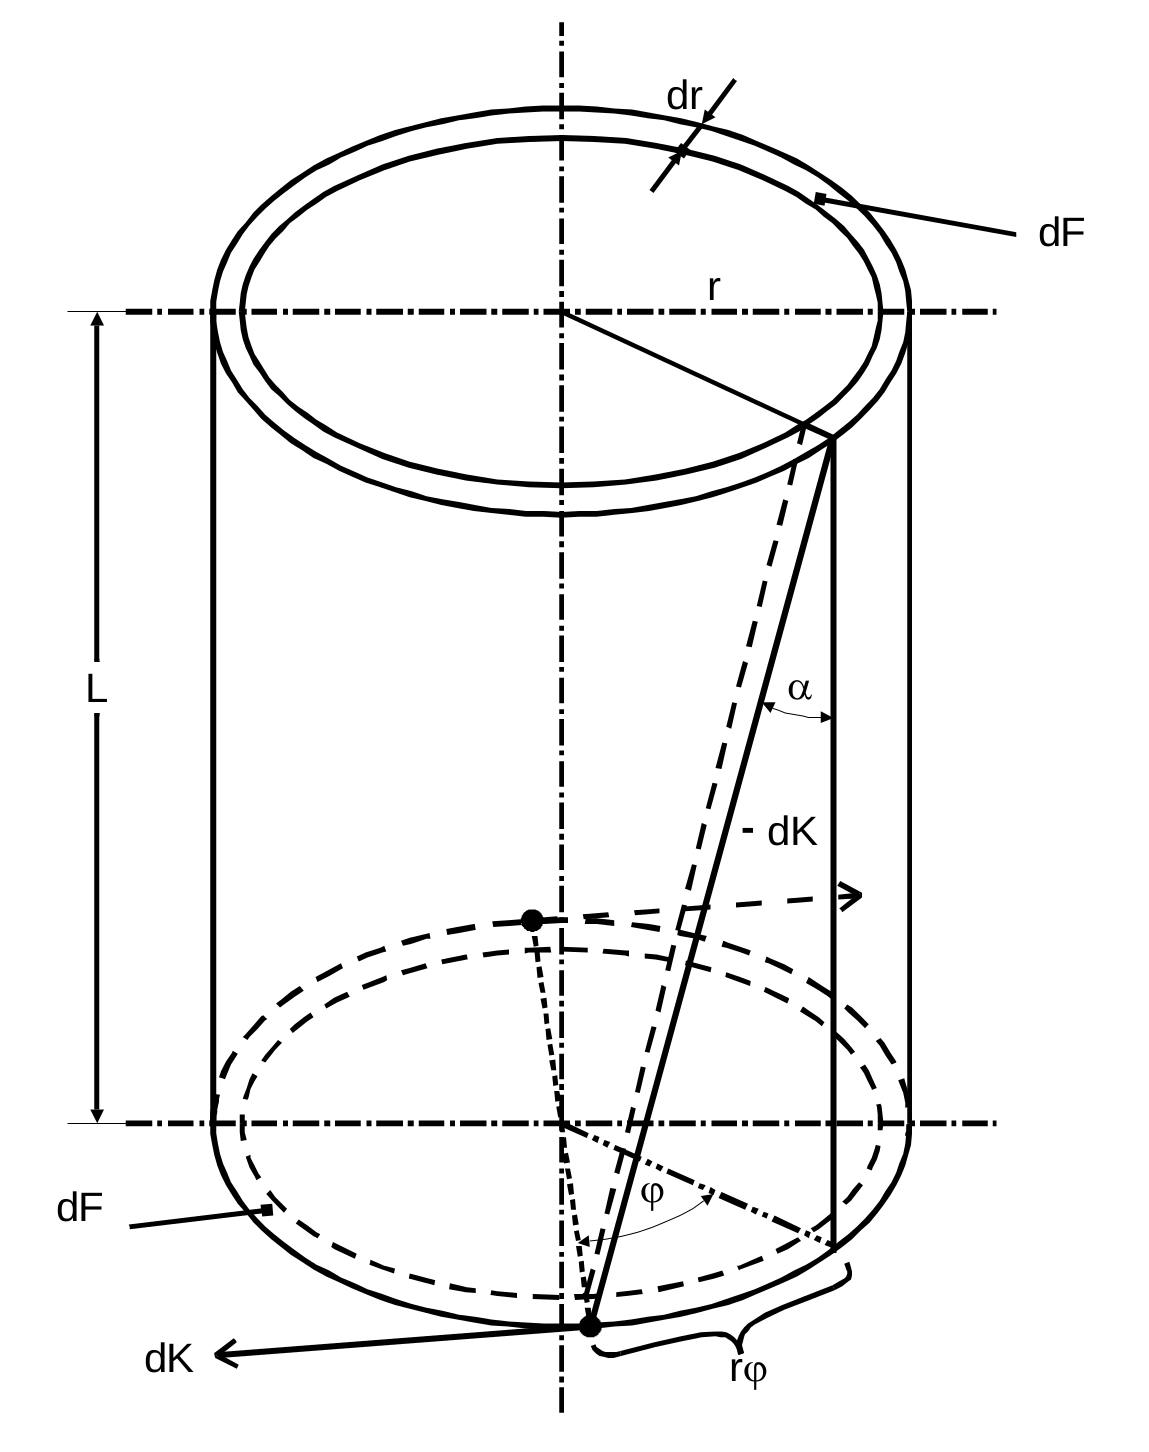
\includegraphics[height=7cm]{content/Zylinder.jpg}
  \caption{Schematische Skizze des verdrillten Zylinders \cite{anleitung}.}
  \label{fig:ZylinderSchema}
\end{figure}

Wird an das untere Ende des Zylinders eine Kugel mit Masse $m_\text{K}$
und Radius $R_\text{K}$
gehängt, so schwingt dieser bei kleiner Verdrillung des Zylinders mit der
Periodendauer
\begin{equation}
    T = 2 \symup{\pi} \sqrt{\frac{\Theta_\text{K} + \Theta_\text{KH}}{D}}.
    \label{eqn:Periodendauer}
\end{equation}
Dabei ist $\Theta_\text{K} = \sfrac{2}{5}\: m_\text{K} R_\text{K}^2$ das
Trägheitsmoment der Kugel und $\Theta_\text{KH}$ das Trägheitsmoment der
Kugelaufhängung. Aus den Gleichungen \eqref{eqn:Periodendauer} und
\eqref{eqn:Richtgröße} ergibt sich somit für den Schubmodul
\begin{equation}
  G = 8 \symup{\pi} \frac{L}{T^2 R^4}
    \left(\frac{2}{5} m_\text{K} R_\text{K}^2 + \Theta_\text{KH}\right).
  \label{eqn:Schubmodul}
\end{equation}

\subsection{Bestimmung des magnetischen Moments}
\label{sec:magTheorie}

Das Produkt aus Polstärke und Abstand der beiden Pole wird magnetisches
Moment $\vec{m}$ eines Permamentmagneten genannt. Wird der Permanentmagnet
in einem homogenen Magnetfeld $B$ um den Winkel $\alpha$ ausgelenkt, gilt für
den Betrag des magnetischen Drehmoments
\begin{equation}
  M_\text{mag} = m B \sin{\alpha}.
\end{equation}
Wird der Aufbau aus Kapitel \ref{sec:TorsionZylinder} verwendet, in ein
homogenes Magnetfeld gebracht und in die Kugel ein Permanentmagnet eingefügt,
so ergibt sich bei kleiner Auslenkung des Systems für die Periodendauer
\begin{equation}
  T_\text{m} = 2 \symup{\pi} \sqrt{\frac{\Theta_\text{K} + \Theta_\text{KH}}{m B + D}}.
  \label{eqn:magPeriode}
\end{equation}
